\chapter{Uvod}

Ovaj završni projekt se izvodi u sklopu projekta FERSAT, koji se od 2018. godine provodi na Fakultetu elektrotehnike i računarstva Sveučilišta u Zagrebu \cite{fersat_stranica_projekta}. Cilj projekta je izrada, lansiranje i korištenje jednog nanosatelita u CubeSat formatu, dimenzija 10 cm x 10 cm x 10 cm, volumena jedne litre i težine ne veće od 4/3 kg. Navedene dimenzije satelita odgovaraju formatu CubeSat 1U. Planirana visina orbite satelita je između 500 i 600 km, a očekivano trajanje misije je 3 godine. Korisni teret satelita (engl. \textit{payload}) se sastoji od tri podsustava:

\begin{itemize}
	\item kamera za snimanje površine Zemlje i zemaljskog horizonta,
	\item detektori svjetla u vidljivom i ultraljubičastom dijelu spektra za mjerenje svjetlosnog onečišćenja i debljine stupca ozona,
	\item komunikacijski sustav u radijskom X-pojasu (10.45 GHz) za prijenos podataka na Zemlju.
\end{itemize}

Kako bi se moglo upravljati radom korisnog tereta, na satelit će biti ugrađeno PDH (engl. \textit{Payload Data Handler}) računalo, čija će zadaća biti prikupljanje podataka s kamere i senzorskog podsustava, pohranjivanje prikupljenih podataka u trajnu memoriju (engl. \textit{non-volatile memory}), te slanje podataka na Zemlju pomoću komunikacijskog sustava. Izabrani mikrokontroler za ulogu PDH računala je STM32L471VGT6 proizvođača ST Microelectronics.

Ostalim podsustavima, koji nisu direktno vezani uz koristan teret, upravlja CDH (engl. \textit{Command and Data Handler}) računalo. CDH računalo može upravljati položajem i orijentacijom satelita, slanjem telemetrijskih podataka na Zemlju, a također upravlja i napajanjem korisnog tereta i šalje naredbe PDH računalu preko CAN (engl. \textit{Controller Area Network}) sučelja. U trenutku pisanja ove dokumentacije, konkretno CDH računalo još nije odabrano.
    
Slika \ref{fig:fersat_blok} prikazuje blok dijagram cijelog sustava. U okviru ovog projekta razvijena je programska potpora PDH računala za upravljanje kamerom i \textit{flash} memorijom.

\begin{figure}[H]
	\centering
	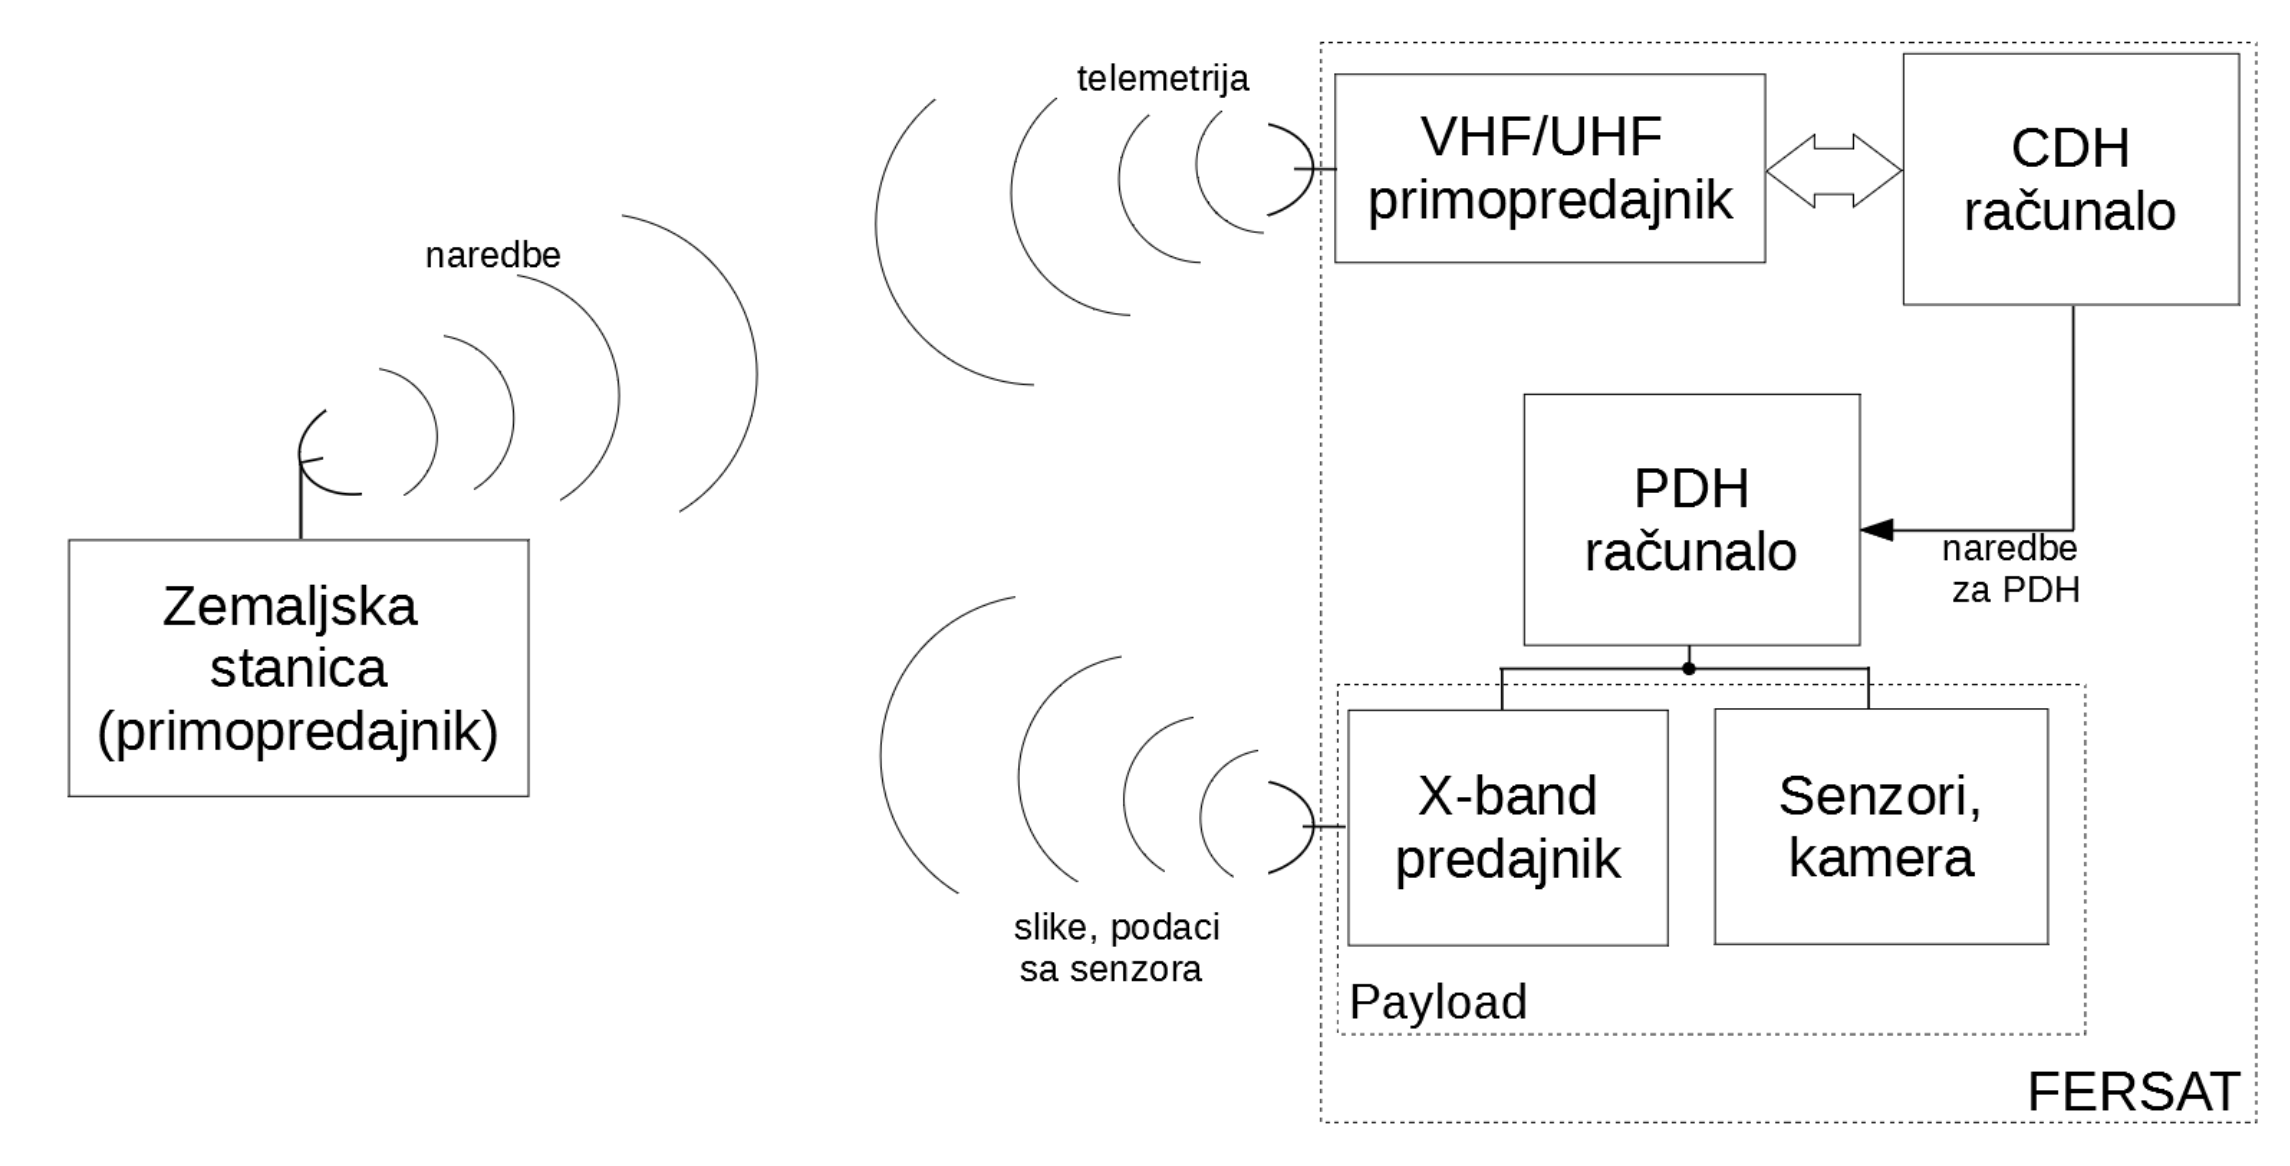
\includegraphics[width=\textwidth]{fersat_blok_dijagram.png}
	\caption{Blok dijagram FERSAT-a i komunikacija sa zemaljskom postajom \cite{diplomski_goran_petrak}}
	\label{fig:fersat_blok}
\end{figure}

Sustav za upravljanje kamerom se sastoji od Arducam Mini 5MP Plus kamere. Upravljanje kamerom se sastoji od konfiguracije kamere i samog korištenja kamere, odnosno slikanja i spremanja slike. Konfiguracija kamere je nužna kako bi se ispravno podesili parametri trajanja ekspozicije, pojačanje i formata u kojem se slika želi spremiti.

\section{Arhitektura sustava}

Slanjem određenog signala na sklop za kameru može se uslikati slika, a nakon slikanja slika se spremi na vlastiti međuspremnik kamere. Cilj je spremljenu kameru pročitati iz međuspremnika kamere i spremiti ju na \textit{flash} memoriju koja se nalazi na pločici PDH-a, gdje može biti spremljena dok se ne zatraži slanje slike preko X-band predajnika na Zemlju.

\textit{Flash} memorija, osim što služi za pohranu slike, služi i za pohranu podataka s drugih senzora. Ona prima i šalje podatke ovisno o poslanoj naredbi putem SPI komunikacije s mikrokontrolerom.

Upravljačko sklopovlje PDH računala se sastoji od STM32F471VGT6 mikrokontrolera, spomenute vanjske \textit{flash} memorije, konektora za povezivanje s ostalim dijelovima sustava (uključujući i konektor za povezivanje s kamerom), sustava za napajanje, upravljačkog sklopovlja za CAN komunikaciju i sklopa za kontrolu izvođenja programa (engl. \textit{watchdog}) \cite{zavrsni_filip_juric}. Izgled tiskane pločice upravljačkog sklopovlja PDH računala prikazan je na slikama \ref{fig:PDH_PCB_1} i \ref{fig:PDH_PCB_2}. Konektor X1 služi za povezivanje sustava s kamerom.

\begin{figure}[H]
	\centering
	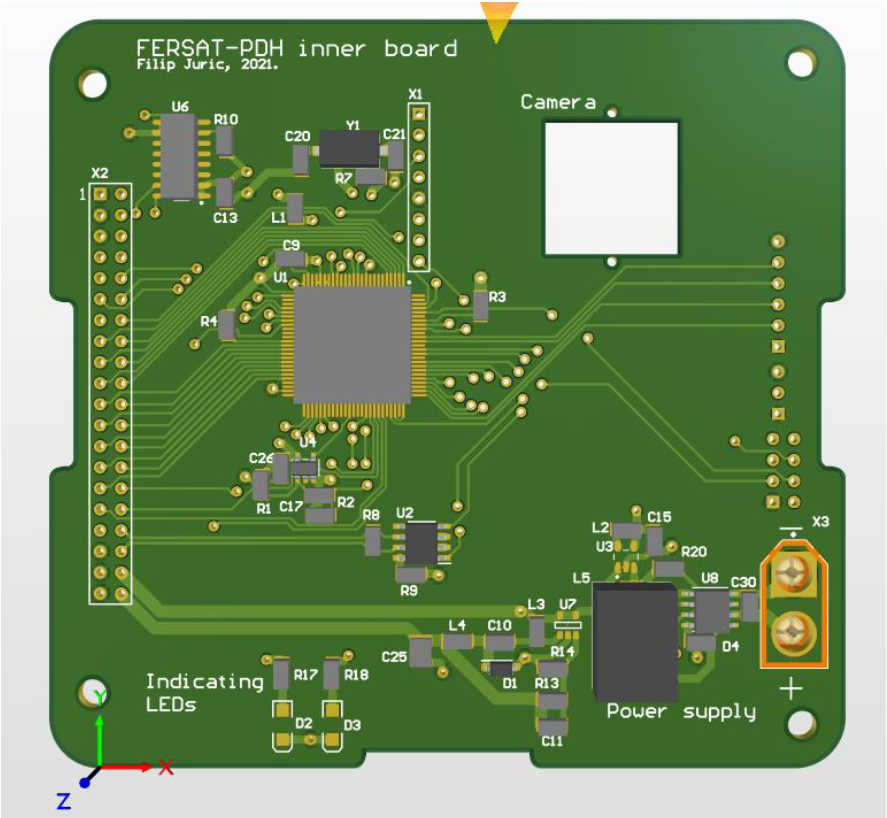
\includegraphics[height= 10 cm]{PDH_PCB_1.PNG}
	\caption{Prikaz gornje strane tiskane pločice upravljačkog sklopovlja PDH računala \cite{zavrsni_filip_juric}}
	\label{fig:PDH_PCB_1}
\end{figure}

\begin{figure}[H]
	\centering
	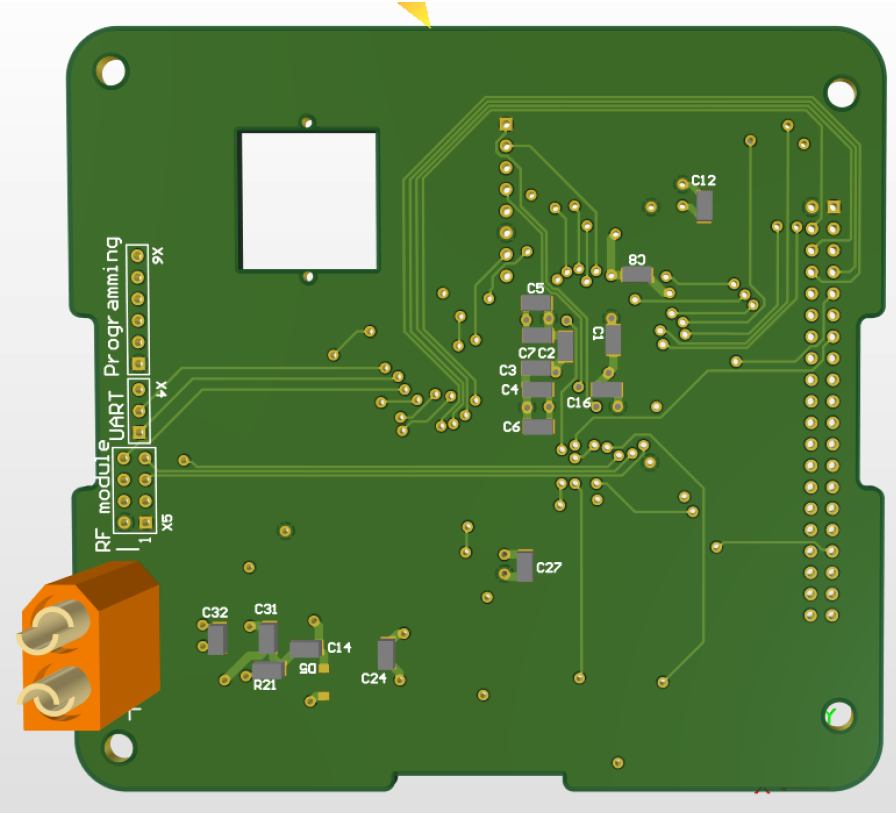
\includegraphics[height= 10 cm]{PDH_PCB_2.PNG}
	\caption{Prikaz donje strane tiskane pločice upravljačkog sklopovlja PDH računala \cite{zavrsni_filip_juric}}
	\label{fig:PDH_PCB_2}
\end{figure}

Programska podrška za PDH računalo već je razvijena \cite{diplomski_goran_petrak}. Međutim, u međuvremenu je došlo do promjene izbora mikrokontrolera PDH računala, te je stoga postojeću programsku podršku bilo potrebno prilagoditi trenutačnom sklopovlju.

S obzirom na prirodu ovog završnog projekta, gdje je naglasak bio na prilagođavanju postojeće programske podrške, u ovom radu će biti raspravljeni izazovi i izmjene do kojih je došlo tijekom prilagođavanja programske podrške. U poglavlju 2 dan je detaljan opis I\textsuperscript{2}C (engl. \textit{Inter-Integrated Circuit}) komunikacije, te su istaknute razlike između starog i novog sklopovlja koje su bile ključne za prilagođavanje programske podrške. Na isti način opisani su SPI (engl. \textit{Serial Peripheral Interface}) komunikacija i DMA (engl. \textit{Direct Memory Access}) prijenos u poglavlju x. Detaljan pregled razvijene programske podrške dan je u poglavlju y, gdje je opisana integracija programske podrške za kameru i \textit{flash} memorija u FreeRTOS operacijski sustav za rad u stvarnom vremenu.